
\documentclass[11pt]{article}
\usepackage[%
  papersize={12.8cm,9.6cm},
  hmargin=1cm,%
  vmargin=1cm,%
  head=0.4cm,% might be changed later
  headsep=0pt,%
  foot=0.5cm% might be changed later
]{geometry}% http://ctan.org/pkg/geometry

\RequirePackage{amsmath}
\RequirePackage{amssymb}
\RequirePackage{amsthm}
%\RequirePackage{algorithmic}
%\RequirePackage{algorithm}
%\RequirePackage{theorem}
%\RequirePackage{eucal}
\RequirePackage{color}
\RequirePackage{url}
\RequirePackage{mdwlist}

\RequirePackage[all]{xy}
\CompileMatrices
\RequirePackage{hyperref}
\RequirePackage{graphicx}
\RequirePackage{relsize}


% xelatex:
\usepackage{fontspec}
\defaultfontfeatures{Ligatures=TeX}
%\usepackage[small,sf,bf]{titlesec}
%\setromanfont{DejaVu Serif}
%\setromanfont{Droid Serif}
%\setromanfont{Gentium} % nice! a bit fluffy
\setromanfont{Gentium Book Basic} % more bold



\RequirePackage{graphicx}
\usepackage{color}
\usepackage{amsfonts}


%\def\heading #1{\vskip 20pt \noindent\underline{\large \bf #1}\vskip 5pt}
\def\heading #1{\centerline{\underline{\bf\LARGE #1}}}
\def\vsp {\vskip 0.5cm}

\def\ket #1{|#1\rangle}
%\def\point {\vskip 5pt $\to$\ \ }
%\def\point {\vskip 5pt $\Longrightarrow$\ \ }
%\def\point {\vskip 5pt $\bigodot$\ \ }
\def\point {\vskip 5pt $\hookrightarrow$\ \ }

\begin{document}

\large

\pagenumbering{gobble}

%%%%%%%%%%%%%%%%%%%%%%%%%%%%%%%%%%%%%%%%%%%%%%%%%%%%%%%%%%%


\centerline{\LARGE }
\vskip 0.5cm
\centerline{\LARGE Distributivity, size, homomorphism}
\vskip 0.5cm
\centerline{\LARGE }

\vskip 1cm

\centerline{\Large Simon Burton}

\vskip 0.5cm

\centerline{School of Physics, The University of Sydney}


%\newpage %%%%%%%%%%%%%%%%%%%%%%%%%%%%%%%%%%%%%%%%%%%%%%%%%%
%
%\begin{center}
%\includegraphics[width=0.2\textwidth]{ExclamationMark.pdf}
%\end{center}
%
%\vskip 0.5cm
%
%\heading{Warning}
%
%My interpretation of quantum physics
%
%The coherence hypothesis

\newpage %%%%%%%%%%%%%%%%%%%%%%%%%%%%%%%%%%%%%%%%%%%%%%%%%%

\heading{Matrix multiplication}

\centerline{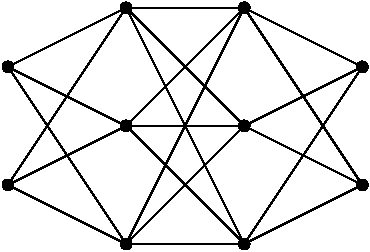
\includegraphics[]{pic-trellis.pdf}}

Distributivity:
$$
    a(b + c) = ab + ac
$$
\vsp\vsp
\vsp\vsp

\newpage %%%%%%%%%%%%%%%%%%%%%%%%%%%%%%%%%%%%%%%%%%%%%%%%%%

\heading{Minimum weight path}
\centerline{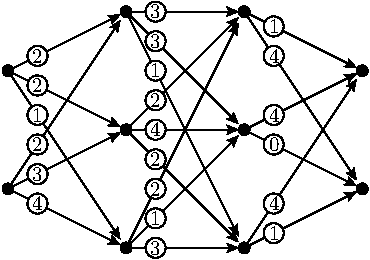
\includegraphics[]{pic-minpath-0.pdf}}
$$
    |\mbox{paths}| = 2.3.3.2 = 36
$$

\newpage %%%%%%%%%%%%%%%%%%%%%%%%%%%%%%%%%%%%%%%%%%%%%%%%%%

\heading{Minimum weight path}
\centerline{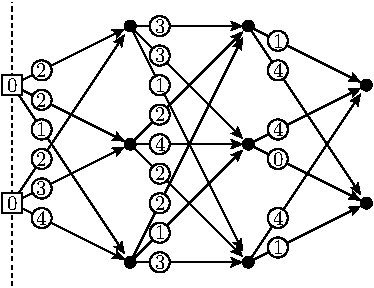
\includegraphics[]{pic-minpath-1.pdf}}

\newpage %%%%%%%%%%%%%%%%%%%%%%%%%%%%%%%%%%%%%%%%%%%%%%%%%%

\heading{Minimum weight path}
\centerline{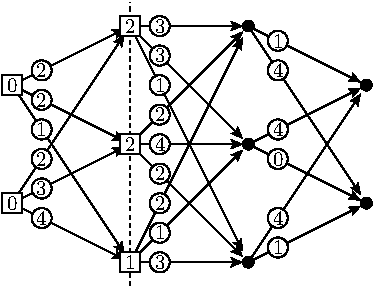
\includegraphics[]{pic-minpath-2.pdf}}

\newpage %%%%%%%%%%%%%%%%%%%%%%%%%%%%%%%%%%%%%%%%%%%%%%%%%%

\heading{Minimum weight path}
\centerline{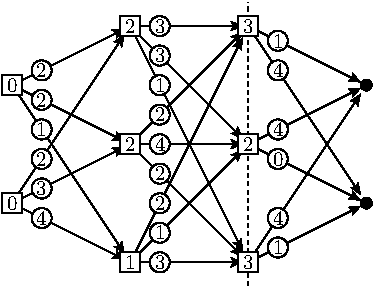
\includegraphics[]{pic-minpath-3.pdf}}

\newpage %%%%%%%%%%%%%%%%%%%%%%%%%%%%%%%%%%%%%%%%%%%%%%%%%%

\heading{Minimum weight path}
\centerline{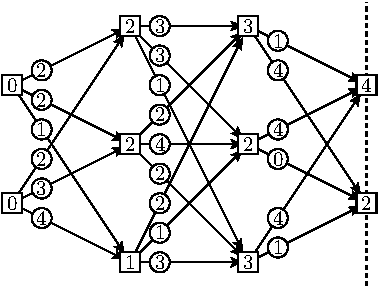
\includegraphics[]{pic-minpath-4.pdf}}

Distributivity:
$$
    a + \min(b, c) = \min(a+b, a+c)
$$

%\newpage %%%%%%%%%%%%%%%%%%%%%%%%%%%%%%%%%%%%%%%%%%%%%%%%%%
%
%\heading{Mailbox Analogy}
%
%\vsp
%The \emph{words} are the key, or the address:
%\begin{center}
%\includegraphics[width=0.3\textwidth]{Key.png}
%\ \ \ \
%\includegraphics[width=0.4\textwidth]{Address.pdf}
%\end{center}
%
%The \emph{meaning} is in the mailbox:
%\begin{center}
%\includegraphics[width=0.4\textwidth]{Mailbox.jpg}
%\end{center}
%
%
%\newpage %%%%%%%%%%%%%%%%%%%%%%%%%%%%%%%%%%%%%%%%%%%%%%%%%%
%
%\heading{Determinism}
%
%%\vsp
%%\centerline{the quest for control}
%
%\begin{center}
%\includegraphics[width=0.4\textwidth]{Clockwork.jpg}
%\end{center}
%
%\begin{center}
%\includegraphics[width=0.4\textwidth]{formula.pdf}
%\end{center}
%
%
%\newpage %%%%%%%%%%%%%%%%%%%%%%%%%%%%%%%%%%%%%%%%%%%%%%%%%%
%
%\heading{Machine Learning}
%
%\vsp\vsp
%
%\vsp\vsp
%\begin{center}
%\includegraphics[width=0.5\textwidth]{GERTY.jpg}
%\end{center}
%
%\vsp\vsp
%Can we find meaning in the machines?
%
%\newpage %%%%%%%%%%%%%%%%%%%%%%%%%%%%%%%%%%%%%%%%%%%%%%%%%%
%
%\heading{Machine Learning}
%
%%Fragile to change in context
%\vsp
%\vsp
%\vsp
%
%\begin{center}
%\includegraphics{function-0.pdf}
%\end{center}
%
%
%\newpage %%%%%%%%%%%%%%%%%%%%%%%%%%%%%%%%%%%%%%%%%%%%%%%%%%
%
%\heading{Machine Learning}
%
%\vsp
%\vsp
%\vsp
%
%\begin{center}
%\includegraphics{function-1.pdf}
%\end{center}
%
%$$
%f(x) = x^4 - 6x^3 + 3x^2 + 10x
%$$
%
%\newpage %%%%%%%%%%%%%%%%%%%%%%%%%%%%%%%%%%%%%%%%%%%%%%%%%%
%
%\heading{Machine Learning}
%
%
%\begin{center}
%\includegraphics{function-2.pdf}
%\end{center}
%
%Fragile to change in context
%
%\newpage %%%%%%%%%%%%%%%%%%%%%%%%%%%%%%%%%%%%%%%%%%%%%%%%%%
%
%\heading{Machine Learning}
%
%\vsp
%\vsp
%\begin{center}
%\includegraphics[width=0.6\textwidth]{AdversarialNoise.png}
%\end{center}
%
%Fragile models
%
%\newpage %%%%%%%%%%%%%%%%%%%%%%%%%%%%%%%%%%%%%%%%%%%%%%%%%%
%
%\heading{Machine Learning}
%
%\vsp\vsp
%\begin{center}
%\includegraphics[width=0.4\textwidth]{StarTrek.jpg}
%\end{center}
%Fragile communication
%
%\newpage %%%%%%%%%%%%%%%%%%%%%%%%%%%%%%%%%%%%%%%%%%%%%%%%%%
%
%\heading{Quantum Contextuality}
%\vsp
%
%\begin{center}
%\includegraphics[width=0.8\textwidth]{two-worlds.pdf}
%\end{center}
%
%\hspace{3 em} Quantum \hspace{9 em} Classical
%
%\newpage %%%%%%%%%%%%%%%%%%%%%%%%%%%%%%%%%%%%%%%%%%%%%%%%%%
%
%\heading{Quantum Contextuality}
%\vsp
%
%\begin{center}
%\includegraphics[width=0.8\textwidth]{two-worlds.pdf}
%\end{center}
%
%\hspace{4 em} Possible \hspace{9 em} Actual
%
%\vsp
%\centerline{There are no causes}
%
%\centerline{Happenings are spontaneous}
%
%
%\newpage %%%%%%%%%%%%%%%%%%%%%%%%%%%%%%%%%%%%%%%%%%%%%%%%%%
%
%\heading{Quantum Contextuality}
%\vsp
%
%\begin{center}
%\includegraphics[width=0.8\textwidth]{two-worlds.pdf}
%\end{center}
%
%\hspace{4 em} Possible \hspace{9 em} Actual
%
%\vsp
%\centerline{Quantum physics is incomplete!}
%
%\newpage %%%%%%%%%%%%%%%%%%%%%%%%%%%%%%%%%%%%%%%%%%%%%%%%%%
%
%\heading{Incompleteness}
%
%\vsp
%\vsp
%\centerline{bug or feature?}
%
%
%\newpage %%%%%%%%%%%%%%%%%%%%%%%%%%%%%%%%%%%%%%%%%%%%%%%%%%
%
%\heading{Incompleteness Is Endemic}
%
%\vsp
%\vsp
%\centerline{Copenhagen (1927)}
%
%\vsp
%\centerline{Wall st. (1929)}
%
%\vsp
%\centerline{G{\"o}del (1931)}
%
%\vsp
%\centerline{Turing (1936)}
%
%
%\newpage %%%%%%%%%%%%%%%%%%%%%%%%%%%%%%%%%%%%%%%%%%%%%%%%%%
%
%\heading{Incompleteness Is Endemic}
%
%\vsp
%\begin{align*}
%\mbox{Copenhagen (1927)} &\longrightarrow \mbox{happenings} \\
%&\\
%\mbox{Wall st. (1929)} &\longrightarrow \mbox{value} \\
%&\\
%\mbox{G{\"o}del (1931)} &\longrightarrow \mbox{mathematical truth} \\
%&\\
%\mbox{Turing (1936)} &\longrightarrow \mbox{computation}
%\end{align*}
%
%\newpage %%%%%%%%%%%%%%%%%%%%%%%%%%%%%%%%%%%%%%%%%%%%%%%%%%
%
%\heading{Entanglement}
%
%\begin{center}
%\includegraphics[width=0.55\textwidth]{entanglement.pdf}
%\end{center}
%\hspace{6.5 em} Possible \hspace{6 em} Actual
%
%
%\newpage %%%%%%%%%%%%%%%%%%%%%%%%%%%%%%%%%%%%%%%%%%%%%%%%%%
%
%%\heading{Entanglement}
%%
%%\begin{center}
%%\includegraphics[width=0.55\textwidth]{entanglement.pdf}
%%\end{center}
%
%\heading{Quantum Physics}
%
%\vsp
%\underline{Contextuality:}
%\vsp
%\centerline{spontaneous (uncaused) happenings.}
%\vsp
%\underline{Entanglement:}
%\vsp
%\centerline{correlations that can only imply non-separation.}
%\vsp
%\underline{Observer:}
%\vsp
%\centerline{left completely undefined.}
%
%\newpage %%%%%%%%%%%%%%%%%%%%%%%%%%%%%%%%%%%%%%%%%%%%%%%%%%
%
%\vsp
%\vsp
%\vsp
%\vsp
%
%\begin{center}
%\includegraphics[width=0.9\textwidth]{dichotomy.pdf}
%\end{center}
%
%
%\newpage %%%%%%%%%%%%%%%%%%%%%%%%%%%%%%%%%%%%%%%%%%%%%%%%%%
%
%\vsp
%\vsp
%\vsp
%\vsp
%
%\begin{center}
%\includegraphics[width=0.9\textwidth]{dichotomy-life.pdf}
%\end{center}
%
%
%\newpage %%%%%%%%%%%%%%%%%%%%%%%%%%%%%%%%%%%%%%%%%%%%%%%%%%
%
%\heading{Order in Physical Systems}
%
%\vsp
%Local order parameter:
%
%\begin{center}
%\includegraphics[width=0.9\textwidth]{magnetic-order.pdf}
%\end{center}
%
%\newpage %%%%%%%%%%%%%%%%%%%%%%%%%%%%%%%%%%%%%%%%%%%%%%%%%%
%
%\heading{Order in Physical Systems}
%
%\vsp
%Topological order:
%
%\begin{center}
%\includegraphics[width=0.9\textwidth]{topological-order.pdf}
%\end{center}
%
%
%\newpage %%%%%%%%%%%%%%%%%%%%%%%%%%%%%%%%%%%%%%%%%%%%%%%%%%
%
%\heading{Other physics}
%
%\vsp\vsp
%Entanglement Harvesting: Summers and Werner, 1987
%
%\vsp\vsp
%Entanglement Purification: Bennett et al. 1995.
%
%
%
%%\newpage %%%%%%%%%%%%%%%%%%%%%%%%%%%%%%%%%%%%%%%%%%%%%%%%%%
%%
%%\heading{The Coherence Hypothesis}
%%
%%\vsp
%%\vsp
%%Living things \underline{are}
%%the (quantum) coherent states (of matter).
%%That is, living systems have access to
%%vast amounts of entanglement.
%%\vsp
%%\vsp
%%In other words: quantum physics is way
%%more relevant than it seems.
%
%\newpage %%%%%%%%%%%%%%%%%%%%%%%%%%%%%%%%%%%%%%%%%%%%%%%%%%
%
%\heading{State Teleportation (1993)}
%
%\begin{center}
%\includegraphics[width=0.5\textwidth]{Teleportation-Coecke.png}
%\end{center}
%Bob Coecke, arXiv:1602.07618
%
%\newpage %%%%%%%%%%%%%%%%%%%%%%%%%%%%%%%%%%%%%%%%%%%%%%%%%%
%
%\heading{State Teleportation}
%
%\begin{center}
%\includegraphics[width=0.55\textwidth]{teleportation.pdf}
%\end{center}
%
%\newpage %%%%%%%%%%%%%%%%%%%%%%%%%%%%%%%%%%%%%%%%%%%%%%%%%%
%
%\heading{Meaning \emph{is} Possibility}
%
%\begin{center}
%\includegraphics[width=0.55\textwidth]{teleportation.pdf}
%\end{center}
%
%\newpage %%%%%%%%%%%%%%%%%%%%%%%%%%%%%%%%%%%%%%%%%%%%%%%%%%
%
%\vsp
%\vsp
%\vsp
%\vsp
%%All differences in this world are of degree, and not of kind, because oneness is the secret of everything.
%``The essence of Vedanta is that there is but one Being and that every soul is that Being in full, not a part of that Being.''
%- Swami Vivekananda
%
%
%\vsp
%``The thought 'Who am I?' will destroy all other thoughts and finally kill itself also.''
%- Sri Ramana Maharshi
%
%
%
%%We are under the incredibly absurd illusion that there is an objective world "outside" Consciousness and there is a "me" inside this body. There is not a shred of truth in these presumption. 
%%
%%You presume you are the body—but, in reality, you are only
%%witnessing the body
%%
%%you are simply the formless and actionless mere witness of
%%whatever is arising
%%
%%
%%If you inspect awareness itself, if you enter into it most profoundly,
%%you will clearly see that awareness itself does not change, but it is
%%(simply and only) the in-depth mere witness of changes.
%%
%%Consciousness Is the "substance" in which all passing phenomena
%%are arising and disappearing.
%
%\vsp
%\vsp
%``No matter what arises, or does not arise,
%there is only Consciousness Itself.''
%- Adi Da Samraj
%

\newpage %%%%%%%%%%%%%%%%%%%%%%%%%%%%%%%%%%%%%%%%%%%%%%%%%%


\end{document} %%%%%%%%%%%%%%%%%%%%%%%%%%%%%%%%%%%%%%%%%%%%%%%%%%%%%%%%%%%

